\documentclass[12pt]{article}
\usepackage[letterpaper, margin=1in]{geometry}

\usepackage{amsmath}
\usepackage{hyperref}
\usepackage{xspace}

\usepackage{graphicx}
\graphicspath{{images/}}

\usepackage{setspace}
\doublespacing

\usepackage[backend=biber,style=ieee,hyperref=true]{biblatex}
\addbibresource{references.bib}

\usepackage{fontspec}
\usepackage{kpfonts}
\fontspec{baskervaldx}
\setmainfont[Numbers=OldStyle]{baskervaldx}
\setmonofont[Scale=.9]{Courier New}

\newcommand{\amp}{\textit{\&}\xspace}

\newcommand{\ac}{\textsc{ac}\xspace}
\newcommand{\am}{\textsc{am}\xspace}
\newcommand{\dc}{\textsc{dc}\xspace}
\newcommand{\rf}{\textsc{am}\xspace}
\newcommand{\ssb}{\textsc{ssb}\xspace}

\DeclareMathOperator{\sign}{sign}

\title{\textsc{On SSB Modulation}}
\author{Catherine Van West}
\date{Autumn, `23}

\begin{document}
\maketitle

\section*{Introduction}
Single-sideband modulation (hereafter \ssb modulation or just \ssb) is a
modulation scheme which decreases the bandwidth use of ordinary amplitude
modulation (\am) by a factor of two \autocite{ssb-thaddeus}. Ordinary \am
implemented using a single mixer produces two sidebands around the carrier
frequency (optionally with a strong component at the carrier itself). Since the
modulating signal is usually purely real, one of these sidebands is redundant
and may be eliminated without loss of information. Additionally, \ssb
modulation often suppresses the carrier, fully or partially, reducing the
amount of power needed to transmit the signal \autocite{weaver-rowell}.

This report examines the mathematics behind \am \amp \ssb, including a few
properties of the Hilbert transform. Basic familiarity with Euler's formula is
assumed. It also gives an overview of a few potential implementations,
including both Hartley and Weaver modulators, and discusses the advantages and
shortcomings of each.

\section*{Mathematics}

\newcommand{\oin}{\omega_\text{in}}
\newcommand{\olo}{\omega_\text{lo}}

To illustrate the behavior of ordinary \am, consider a sinusoidal signal \(s(t)
= \cos \omega t\). Using Euler's formula, \(e^{jt} = \cos t + j \sin t\), we
may represent this as \(s(t) = \frac 1 2 (e^{j \omega t} + e^{- j \omega t})\).
Note that a single real sinusoid consists of two complex sinusoids at positive
and negative frequencies. If a baseband signal \(\cos \oin t\) is mixed with a
carrier signal \(\cos \olo t\), the result is
\begin{align*}
	\left(\cos \oin t\right) \left(\cos \olo t\right)
		&= \frac 1 2 \left(e^{j \oin t} + e^{-j \oin t}\right)
			\cdot \frac 1 2 \left(
				e^{j \olo t} + e^{-j \olo t}
			\right) \\
		&= \frac 1 4 \left(
			e^{j (\olo \pm \oin) t} + e^{-j (\olo \pm \oin) t}
		\right) \\
		&= \frac 1 2 \cos (\olo \pm \oin) t.
\end{align*}
The modulated signal contains frequency components both above and below the
carrier, although these both have the same information content. The results of
modulation are illustrated in figure \ref{fig:razavi-am}.

\begin{figure}[h]
	\centering
	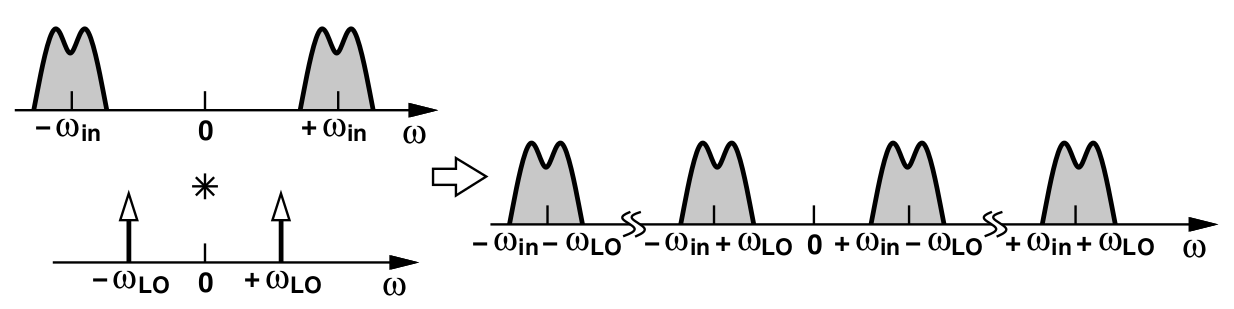
\includegraphics[width=.9\textwidth]{razavi-am.png}
	\caption{Amplitude modulation of a baseband signal
	\autocite{rf-microelectronics}.}
	\label{fig:razavi-am}
\end{figure}

The mathematical means of suppressing one of the sidebands is using the Hilbert
transform. The Hilbert transform is equivalent to a filter with transfer
function \(H(\omega) = -j \sign \omega\). Applying this filter to a  sinusoid
\(\cos \omega t = \frac 1 2 (e^{j \omega t} + e^{-j \omega t})\) yields \(\frac
1 2 (-j e^{j \omega t} + j e^{-j \omega t}) = \sin \omega t\) -- in other
words, taking the Hilbert transform of a signal shifts all real frequency
components by \(\frac \pi 2\). For \ssb, the baseband signal is modulated twice
-- once in its original form, and once after passing it through a Hilbert
transformer \autocite{ssb-tretter}.

If this process is applied to the same sinusoidal signals as above, yielding
\(s(t) = \cos \oin t \) and its Hilbert transform \(\hat s(t) = \sin \oin t\).
These signals are then modulated with \(\cos \olo t\) and \(\sin \olo t\),
respectively, to produce in-phase and quadrature components of the output:
\begin{align*}
	I(t) &= s(t) \cos \olo t \\
		&= \frac 1 4 \left(
			e^{j (\olo \pm \oin) t} + e^{-j (\olo \pm \oin) t}
		\right) \text{ by the above, and} \\
	Q(t) &= \hat s(t) \sin \olo t \\
		&= \frac 1 2 \left(-j e^{j \oin t} + j e^{-j \oin t}\right)
			\cdot \frac 1 2 \left(
				-j e^{j \olo t} + j e^{-j \olo t}\right
			) \\
		&= \frac 1 4 \left(
			-e^{\pm j (\oin + \olo) t} + e^{\pm j (\oin - \olo)}
		\right) \text { after distributing.}
\end{align*}
Note that, although expressed in terms of complex sinusoids, both \(I(t)\) and
\(Q(t)\) are \emph{real} signals; the process above may be implemented in
analog hardware. Sideband selection is performed by either adding or
subtracting \(I(t)\) and \(Q(t)\) -- for example, adding yields
\begin{align*}
	I(t) + Q(t) &= \frac 1 4 \left(
		2 e^{j (\olo - \oin) t} + 2 e^{-j (\olo - \oin) t}
	\right) \\
	&= \cos (\olo - \oin) t \text{ after canceling \(\pm \sin\),}
\end{align*}
leaving only the lower sideband.

Demodulation functions as modulation in reverse -- the \rf signal is multiplied
by in-phase and quadrature components of a local oscillator, inverse Hilbert
transformed, then added back together to form the baseband signal. The Hartley
architecture is one example implementation, used since the early days of radio;
the Weaver architecture is another \autocite{rf-microelectronics}.

\printbibliography

\end{document}
